\documentclass[14pt]{beamer} %Makes presentation
%\documentclass[14pt, handout]{beamer} %Makes Handouts

\setbeamercolor{normal text}{fg=white,bg=blue!20!black}
\setbeamercolor{structure}{fg=white, bg=blue!20!black}
\setbeamercolor{alerted text}{fg=yellow!70!orange}
%\setbeamercolor{item projected}{use=item,fg=black,bg=item.fg!35}
\setbeamercolor*{palette primary}{use=structure,fg=structure.fg}
\setbeamercolor*{palette secondary}{use=structure,fg=structure.fg!95!black}
\setbeamercolor*{palette tertiary}{use=structure,fg=structure.fg!90!black}
\setbeamercolor*{palette quaternary}{use=structure,fg=structure.fg!95!black,bg=black!80}
\setbeamercolor*{framesubtitle}{fg=white}
\setbeamercolor*{block title}{use=structure, bg=blue!20!black}
\setbeamercolor*{block body}{use=structure}

\setbeamertemplate{navigation symbols}{}
%\setbeamertemplate{mini frames}[default]
%\setbeamercovered{dynamics}
\setbeamerfont*{title}{size=\Large,series=\bfseries}

%\setbeameroption{notes on second screen} %Dual-Screen Notes
%\setbeameroption{show only notes} %Notes Output

\setbeamertemplate{frametitle}{\vspace{.5em}\bfseries\insertframetitle}
\newcommand{\heading}[1]{\noindent \textbf{#1}\\ \vspace{1em}}

% small footnotes
\setbeamerfont{footnote}{size=\tiny}

\usepackage{bbding,color,multirow,times,ccaption,tabularx,graphicx,verbatim,booktabs,fixltx2e}
\usepackage{colortbl} %Table overlays
\usepackage[english]{babel}
\usepackage[latin1]{inputenc}
\usepackage[T1]{fontenc}
\usepackage{lmodern}
\usepackage{alltt}

\usepackage{tikz}
\usetikzlibrary{positioning}
\usetikzlibrary{trees}




\author[]{Thomas J. Leeper}
\institute[]{
  \inst{}%
  Department of Government\\London School of Economics and Political Science
}

\title{\large Presentations: A Presentation}

\date[]{01 March 2018}

\begin{document}

\frame{\titlepage}

\frame{

    \begin{center}
    {\huge
    \onslide<2->{Presenting $\neq$ talking!}
    
    \vspace{1em}
    
    \onslide<2->{Presenting $\neq$ reading!}
    }
    \end{center}

}

\frame{}
\section{Basics}
\frame{\Huge\begin{center}Basics\end{center}}



\frame{

\frametitle{Presentations in a Nutshell}

\large

\begin{enumerate}\itemsep1em
\item Know your audience, why you're talking, and why they're listening
\item Convey one and only one main point
\item Less is almost always more
\end{enumerate}

}


\frame{

\frametitle{Structure of an Academic Talk}

\begin{enumerate}\itemsep1em
\item What are you doing? And why should we care?
\item What do we already know? (Briefly!)
\item What do you think is going on?
\item What did you do?
\item What did you find? And why should we care?
\end{enumerate}

}

\frame{

\frametitle{Structure of a Proposal Talk}

\begin{enumerate}\itemsep1em
\item What are you doing? And why should we care?
\item What do we already know? (Briefly!)
\item What do you think is going on?
\item What \textit{do you plan to} do?
\item \textit{What do you want feedback on?}
\end{enumerate}

}



\frame{}
\section{Slides}
\frame{\Huge\begin{center}Slides\end{center}}


\frame{

\begin{center}
\large
Slides are something you produce for ideas you can't express in spoken word!

\vspace{1em}


Or, they are to emphasize something you are doing as part of the presentation.

\end{center}

}



\frame{

\begin{columns}
\begin{column}{0.5\textwidth}
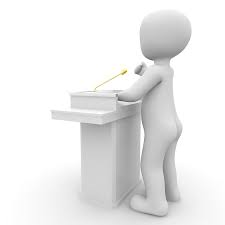
\includegraphics{images/lecture.png}
\end{column}

\begin{column}{0.5\textwidth}
Why is this picture here?

\vspace{1em}

\onslide<2->{Also, the resolution is too low}
\end{column}
\end{columns}
}


\frame{

\frametitle{This is a terrible slide}

\small

\begin{itemize}
\item The bullet points are not really bullet points but extremely long essay-style sentences that no is going to read. The only reason they're here is probably because the presenter thought they might read them out loud from the overhead because they didn't practice and therefore thought they would forget what they were supposed to talk about.
\item To fit all of that text on the slide, the font size is tiny. It's unreadable in fact even at a short distance. What was the presenter thinking?
\item What's the point of this slide ultimately? Is the content on the slide important --- something the audience actually needs to see? Or is the content of this slide here just to reminder the presenter of something? If it's the former, it's failing. If it's the latter, it shouldn't be a slide at all.
\end{itemize}

}


\bgroup
\setbeamercolor{background canvas}{bg=white}
\begin{frame}[plain]{}

\vspace{2em}
\textcolor{black}{\Huge \textbf{\textit{Keep it simple}}}

\vspace{5em}
\onslide<2->{\textcolor{black}{Use contrasting color and font for emphasis.}}
\end{frame}
\egroup



\frame{

\frametitle{How to Use Slides}

\begin{itemize}\itemsep1em
\item Write your presentation. Then make slides.
\item<2-> Keep slides as simple as possible
	\begin{itemize}
	\item Use handouts if necessary
	\end{itemize}
\item<3-> Use large, consistently sized sans-serif fonts
\item<4-> Use clear, high-contrast colors
\item<5-> Use images to convey ideas, not decoration
\end{itemize}

}


\frame{}
\section{Avoiding Mistakes}
\frame{\Huge\begin{center}Avoiding Mistakes\end{center}}


\frame{

\frametitle{Biggest Mistakes}

\begin{itemize}\itemsep1em
\item Reading from slides
\item Reading from bad slides
\item Slide content that you don't talk about
\item Speaking too fast
\item Speaking too quietly
\item Moving around without purpose
\end{itemize}

}

\frame{

\frametitle{Avoiding Mistakes I}

\begin{itemize}\itemsep1em
\item<2-> Practice
\item<3-> Practice
\item<4-> Practice
\item<5-> Practice
\item<6-> Practice
\end{itemize}

}

\frame{

\frametitle{Avoiding Mistakes II}

\begin{itemize}\itemsep1em
\item<2-> Know your time limit. Max 1 slide per minute.
\item<3-> Stop talking when time is up. Don't talk faster.
\item<4-> You don't need to say all your thoughts.
\item<5-> Great artists steal.
\end{itemize}

}

\frame{

\frametitle{Avoiding Mistakes III}

Warm up your voice!

\vspace{3em}

\only<2>{uh --- eh --- ee --- oo --- uu}

\only<3>{To sit in solemn silence in a dull dark dock\\
In a pestilential prison with a life long lock\\
Awaiting the sensation of a short sharp shock\\
From a cheap and chippy chopper on a big black block}

\only<4>{Betty Botter bought some butter, but she said `This butter's bitter.' `If I put it in my batter, it will make my batter bitter.' So, she bought some better butter, better than the bitter butter. When she put it in her batter, the butter made her batter better.}
}



\bgroup
\setbeamercolor{background canvas}{bg=black}
\setbeamertemplate{navigation symbols}{}
\begin{frame}[plain]{}
\end{frame}
\egroup

\section{Example Presentation}

\frame{
\begin{center}
\huge Are Political Orientation Genetically Transmitted?
\end{center}
}


\frame{

\frametitle{Causes of Opinion Formation}

Political scientists have identified many causes of opinion formation:

\begin{itemize}
\item Socialization
\item Mass media
\item Values and predispositions
\end{itemize}

Why haven't we thought about genetics?

}

\frame{

\frametitle{Twin Studies}

\begin{itemize}\itemsep1em
\item Gather phenotype data on pairs of twins
	\begin{itemize}
	\item Monozygotic
	\item Dizygotic
	\end{itemize}
\item Partition outcome variance into three components
	\begin{itemize}
	\item Heritability
	\item Shared environment
	\item Unshared environment
	\end{itemize}
\end{itemize}

}


\frame{

\frametitle{Our Data}

\begin{itemize}\itemsep1em
\item Data:
	\begin{itemize}
	\item Survey of pairs MZ and DZ twins (US)
	\item Supplemental data from Australia
	\end{itemize}
\item Outcome
	\begin{itemize}
	\item Wilson-Patterson Attitude Inventory
	\item 50 items measuring liberal--conservative ideology
	\end{itemize}
\item Method of analysis
	\begin{itemize}
	\item Standard twin study design
	\item Estimate heritability of each issue-specific phenotype and overall ideology
	\end{itemize}
\end{itemize}

}

\frame{

\frametitle{Desired Feedback}

\begin{itemize}\itemsep1em
\item What literature should we situate this in?
	\begin{itemize}
	\item Application of behavioural genetics in new domain
	\item A critique of the political socialization literature
	\end{itemize}
\item How can we improve our measure of political orientations?
\item How can we avoid being seen as advancing a eugenics-type argument?
\end{itemize}

}



\bgroup
\setbeamercolor{background canvas}{bg=black}
\setbeamertemplate{navigation symbols}{}
\begin{frame}[plain]{}
\end{frame}
\egroup

\end{document}
